\chapter{Réalisation}

\section*{Introduction}
 \qquad Une fois nous avons fixé les grandes lignes de notre application et les pilonnes conceptuelles sur les niveaux global et détaillé nous pouvons passer à l'implémentation des modèles théoriques. Pour ce faire, nous allons choisir l'environnement de développement ainsi que les technologies nécessaires. Nous passons à la fin de ce chapitre à la présentation de quelques scénarios d'exécution à travers les interfaces Homme/Machine.
 
 \section{Environnement de travail}
 
\qquad Cette partie s'intéresse à l'environnement logiciel et matériel avec lequel nous avons mené notre projet.  

\subsection{Environnement physique}

\qquad Nous présentons dans ce paragraphe les équipements utilisés durant toutes les phases du projet : Développement, Débogage et Test unitaire. Le tableau \ref{tab4.1} présente la fiche technique des appareils utilisés.

\begin{table}[!h]
	\caption{Fiche technique des équipements utilisés}
	\label{tab4.1}
	\begin{center}
		\begin{tabular}{|L{5cm}|L{5cm}|}
			\hline
			\textbf{Ordinateur} & \textbf{Smartphone}\\
			- Modèle: Asus & - Modèle: Samsung Galaxy S5\\
			- Processeur: Intel i7 & - Processeur: Quad-core 2.5 GHz Krait 400\\
			- Mémoire: 12 GB RAM & - Mémoire: 2 GB RAM\\
			- Stockage interne: 1TB HDD & - Stockage interne: 16 GB\\
			- SE: WINDOWS 10  & - SE: Android 4.4.2\\
			\hline			
		\end{tabular}
	\end{center}
\end{table} 
\newpage
\subsection{Environnement logiciel}

\qquad Après la spécification des environnements physiques nécessaires à la réalisation, nous pouvons passer au choix de l'environnement logiciel. Les différents outils logiciels utilisés durant le stage pour la réalisation des fonctionnalités et la rédaction du rapport sont listés ci-après: 

\begin{itemize}
	\item \textbf{Eclipse}: Environnement de développement intégré (EDI) destiné principalement au développeur JAVA mais il est extensible vers d'autres langages tels que C/C++, PHP et plein d'autres. Nous pouvons combiner plusieurs langages sous un seul EDI à travers les plugins comme nous pouvons avoir un EDI pour chaque objectif. Nous avons utilisé Eclipse dans sa version destinée pour le Java Enterprise Edition durant le projet.
	
	\item \textbf{Visual Studio Code} : Éditeur de code source léger mais puissant qui fonctionne sur bureau et est disponible pour Windows, MacOS et Linux. Il est livré avec un support intégré pour JavaScript, TypeScript et Node.js et dispose d'un riche écosystème d'extensions pour d'autres langues (C ++, C \#, Python, PHP, Go).
	
	\item \textbf{BitBucket} : Gestionnaire de versions distribuées qui permet à une équipe de coopérer ensemble dans un projets large.
	
	\item \textbf{JIRA}: Gestionnaire de taches dans une équipe de travail. Il fournit un tableau de bord pour pouvoir gérer les story dans un environnement de développement SCRUM.
	
	\item \textbf{Confluence}: Logiciel de Wiki qui permet de rédiger la documentation sur le code source délivré.
	
	\item \textbf{PowAMC}: Environnement logiciel destiné à la conception UML. 
	
	\item \textbf{TeXStudio}: Éditeur de texte pour la rédaction des documents en Latex.
\end{itemize}

\section{Choix technologiques}

\qquad Cette partie s'intéresse aux choix des technologies et langages de programmation que nous allons utiliser pour parvenir à la finalité de notre projet comme le montre la figure \ref{fig4.1}.

\begin{figure}[!h]
	\begin{center}
		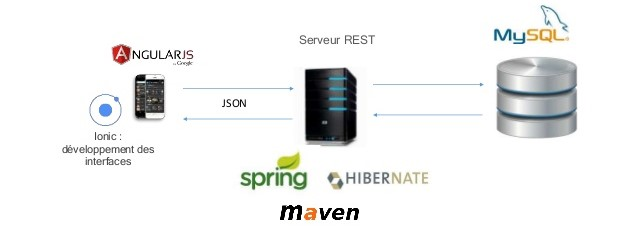
\includegraphics[width=0.64\textheight]{figures/archi}
	\end{center}
	\caption{Technologies utilisées}
	\label{fig4.1}
\end{figure}
\newpage
\begin{itemize}
	\item \textbf{HTML} : langage de balisage crée et utilisé pour écrire les pages Web.
	\item \textbf{CSS} : langage permettent de définir des règles appliquées à un ou plusieurs documents.
	\item \textbf{AngularJS} : Frame-work Javascript open-source, développé par Google, permettant de réaliser des applications Web dynamique en utilisant le modèle MV-VM (Model-View View-Model).
	\begin{itemize}
		\item \textbf{AngularUI Router} : Framework AnguarJS permettant de rajouter un router à la single page application en utilisant des vues imbriquées.
	\end{itemize}
	\item \textbf{Ionic} : Frame-work de développement d'applications hybrides. Ce frame-work permet de développer des applications mobiles pour divers différents environnements d'appareils téléphoniques (Android, Ios et WindowsPhone) en combinant à la fois les technologies Web (HTML, CSS et JavaScript) et les technologies de développement natives des différents environnements (Java SDK, Swift, Objective C ...)\cite{3}.
	\item \textbf{Java Enterprise Edition} : Extension du Java SE contenant des bibliothèques destinée au développement des applications Web robustes.
	\begin{itemize}
		\item \textbf{Jax-RS} : Spécification standard JEE qui fournit les méthodes du protocole HTTP pour pouvoir effectuer des appels REST. Ce standard est indépendant du format des données et est basé sur les POJO.
		\item \textbf{JPA} : API qui permet le mapping relationnel des objets Java sur les classes persistantes de la base de données, utilisé pour interroger la base lors des transactions faites par soit les utilisateurs soit par l'administrateur\cite{6}.
		\item \textbf{JDBC} : Bibliothèque qui permet l'accès au driver de la base de données. Cette bibliothèque est utilisée majoritairement dans les transactions faites lors des traitements par lots (Batch) car elle présente une légèreté de lors de l'interrogation de la base des données.
		\item \textbf{Spring Batch} : Premier Framework Java pour les traitements par lots. La framewrk offre un type par défaut de traitement Batch appelé Job où le job est composé de trois step: Read, Process et Write. Un autre type offert par la framework appelé tasklet offre la possiblité de personnaliser le traitement et d'ajouter autant d'étape que l'on veut à un traitement Batch. Nous avons opté pour le deuxième type parce que la plupart des traitements par lots de notre projet ne présente pas des étapes de lecture ni d'écriture \cite{4} (voir figure \ref{fig4.2}).
		\item \textbf{Apache POI}: Bibliothèque permettant de créer des fichiers Microsoft Office (XLS, Docx, PPT, ...)
		\item \textbf{StreamingOutput}: Bibliothèque permettant de télécharger (Donwnload) des fichier en streaming.  
		\item \textbf{Maven} : Gestionnaire de paquets pour l'environnement JEE.
	\end{itemize}  
	\item \textbf{MySQL} : Système de gestion de base de données relationnelles.
	\item \textbf{ServicesWeb REST} : Exposent entièrement les services comme un ensemble de ressources (URI) identifiables et accessibles par la syntaxe et la sémantique du protocole	HTTP
\end{itemize}

Ci-dessous est représenté un schéma descriptif des principales éléments qui constituent une application faisant appel à un traitement par lots. Généralement, l'architecture est réalisée en trois couches (voir figure \ref{fig4.2}):
\begin{itemize}
	\item Application mère ou couramment appelé projet parent qui contient tous les sous projets en particulier l'application Batch.
	\item Batch Core qui est la couche concernée par le lancement, la surveillance et la gestion des Batch.
	\item Batch infrastructure est la dernière couche qui fournit des API telles que la lecture, le processing et l'écriture des données.  
\end{itemize}
\begin{figure}[!h]
	\begin{center}
		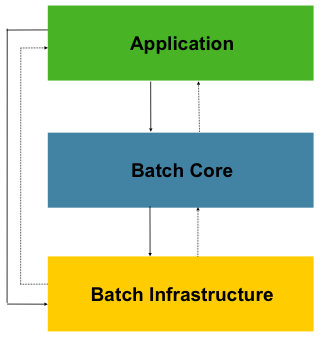
\includegraphics[height=4.5cm]{figures/batch_app}
	\end{center}
	\caption{Relation entre l'application serveur et les applications Batch}
	\label{fig4.2}
\end{figure}


\section{Scénarios d'exécution}

\qquad Ce paragraphe est consacré à la description de quelques scénarios d'exécution à travers les interfaces Homme/Machine fournies par l'application.

\subsection{Partie: Utilisateur}

\qquad L'utilisateur a un accès à l'application à travers une IHM sur son propre appareil téléphonique (smartphone). $\grave{A}$ l'entrée, l'application demande l'utilisateur de connecter son smartphone à Internet pour pouvoir récupérer les données du serveur comme l'indique l'interface \ref{fig4.3}.

\begin{figure}[!h]
	\begin{center}
 		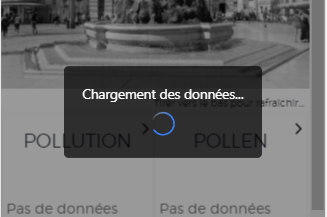
\includegraphics[width=7cm]{figures/Capture1}
 	\end{center}
 	\caption{Récupération des données}
 	\label{fig4.3}
\end{figure}
\newpage
Après avoir récupérer les données, l'application aura besoin de la région désirée. L'utilisateur peut alors, soit activer le service de géolocalisation, soit saisir le code ou le nom de la région comme le montre les exemples de la figure \ref{fig4.4}.

\begin{figure}[!h]
	\begin{center}
		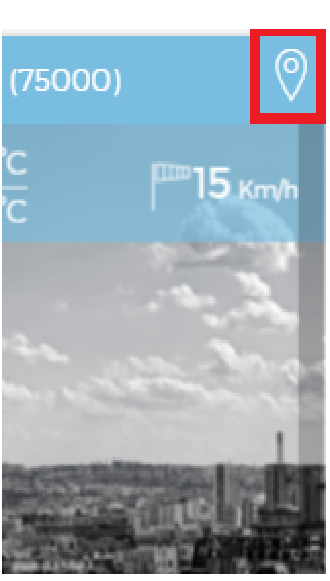
\includegraphics[width=5.25cm]{figures/gps}
		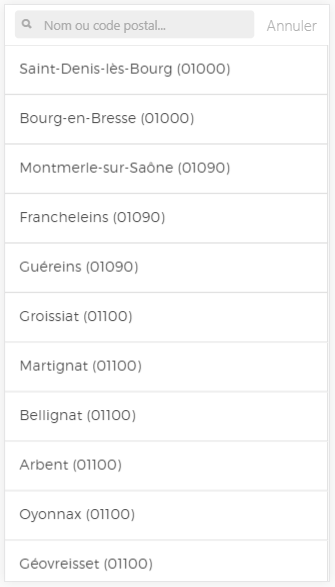
\includegraphics[width=5cm]{figures/choix_ville}
	\end{center}
	\caption{Indication de la ville : Par Service GPS / Par recherche}
	\label{fig4.4}
\end{figure}

Une fois l'application a pu se connecter à Internet et localiser l'utilisateur elle peut maintenant afficher les niveaux des risques auxquels l'utilisateur est abonné (voir figure \ref{fig4.5}).

\begin{figure}[!h]
	\begin{center}
		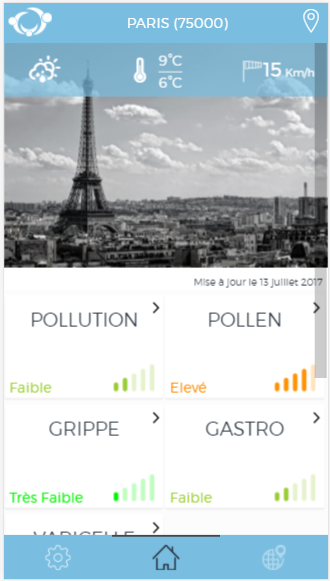
\includegraphics[width=4.6cm]{figures/dash_board}
	\end{center}
	\caption{Consultation des niveaux des risques}
	\label{fig4.5}
\end{figure}
\newpage
L'utilisateur peut aussi consulter des détails et des conseils relatives aux risques (voir figure \ref{fig4.6}) en cliquant sur le risque désiré.

\begin{figure}[!h]
	\begin{center}
		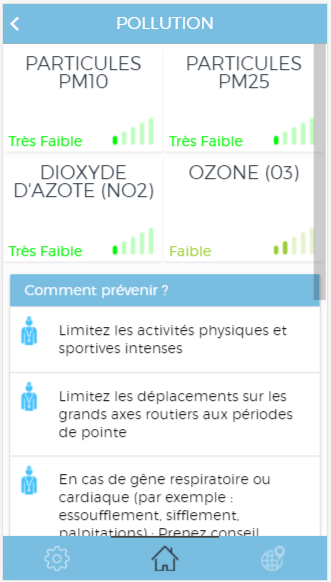
\includegraphics[width=5cm]{figures/detail_risk}
	\end{center}
	\caption{Consultation des détails et des conseils relatives à la pollution}
	\label{fig4.6}
\end{figure}

L'application offre encore la possibilité d'ajouter des astuces à l'application. Dans le menu principal, L'utilisateur peut faire descendre l'écran vers le bas, il trouvera alors la section intitulée "pense bête" où est affiché un message aléatoire relatif au risque ayant le plus haut niveau (voir figure \ref{fig4.7}).

\begin{figure}[!h]
	\begin{center}
		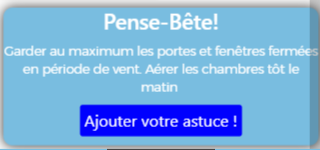
\includegraphics[width=7cm]{figures/pense_bete}
	\end{center}
	\caption{Section: Pense Bête}
	\label{fig4.7}
\end{figure}
\vspace{1cm}
En cliquant sur le bouton "Ajouter votre astuce", une popup s'affiche, comme le montre la figure \ref{fig4.8}, donnant ainsi la possibilité de remplir les informations qui concernent l'astuce ajoutée (Pseudonyme du contributeur, Adresse mail, Type de risque et Texte de l'astuce).

\begin{figure}[!h]
	\begin{center}
		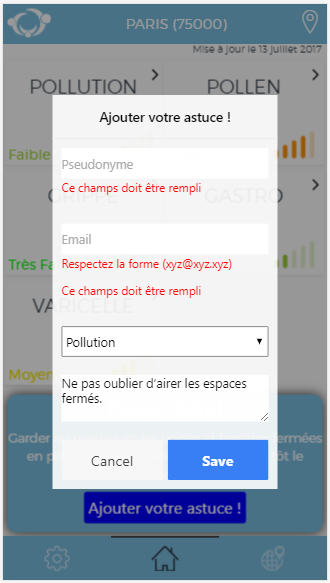
\includegraphics[height=8cm]{figures/ajout_trick}
	\end{center}
	\caption{Popup: Ajout d'astuces}
	\label{fig4.8}
\end{figure}
\newpage
La figure \ref{fig4.8} montre aussi le cas échéant où l'utilisateur saisit incorrectement les informations demandées. Au cas où les informations sont absentes ou incorrectes, un message d'erreur est affiché sous chaque champ erroné.

\vspace{0.5cm}

$\grave{A}$ la réception d'une notification, l'application navigue vers une interface où l'utilisateur peut choisir parmi trois conseils qui lui seront envoyé à chaque pique de niveau du risque en question. En cliquant sur le bouton "Enregistrer", il enregistre ses choix et retourne vers le menu principal (voir figure \ref{fig4.9}).

\begin{figure}[!h]
	\begin{center}
		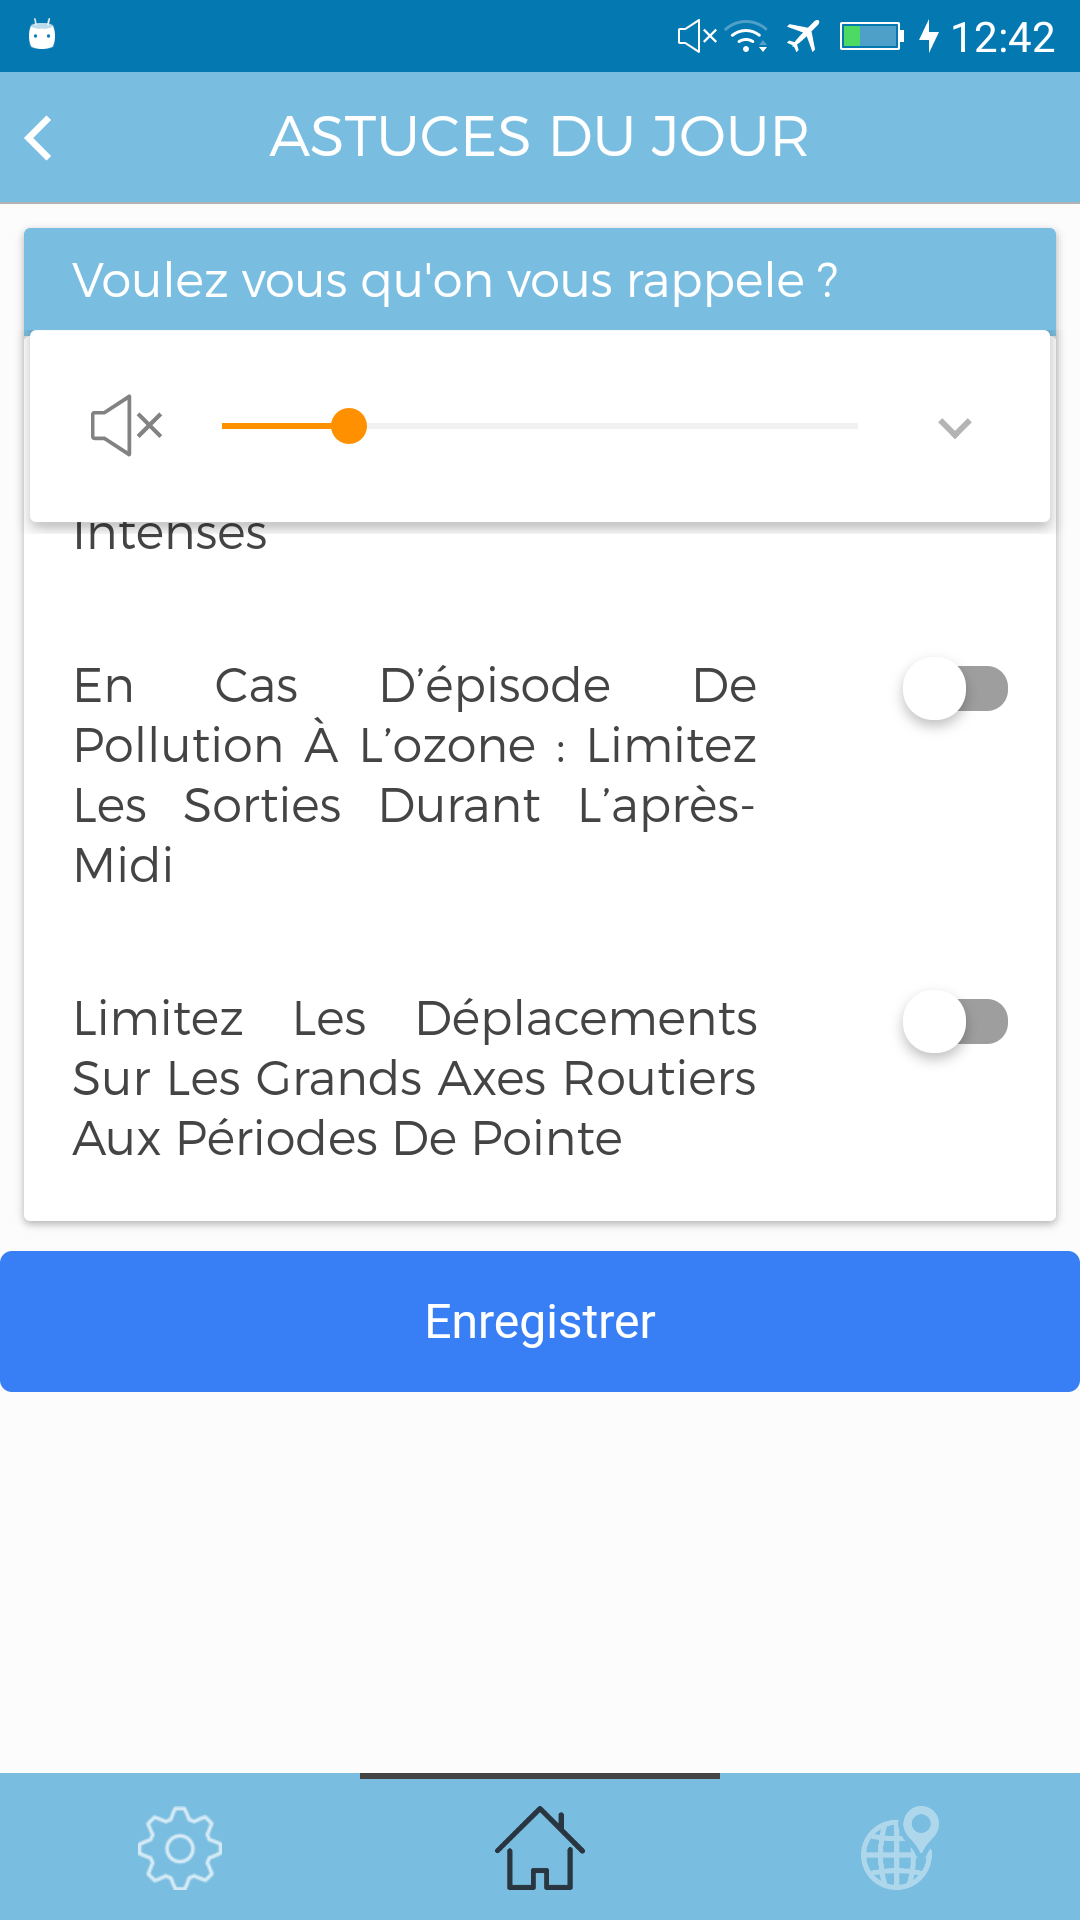
\includegraphics[height=8cm]{figures/rappel_trick}
	\end{center}
	\caption{Choix des astuces "Pique des niveaux des risques"}
	\label{fig4.9}
\end{figure}

 L'utilisateur consulte la rubrique configuration pour paramétrer l'application (voir figure \ref{fig4.10}). Cette dernière accorde à l'utilisateur plusieurs fonctionnalités: 
\begin{itemize}
	\item S'abonner et/ou se désabonner d'un risque
	\item Permettre l'accès aux données personnelles (position géographique)
	\item S'abonner ou se désabonner aux notifications
\end{itemize} 

\begin{figure}[!h]
	\begin{center}
		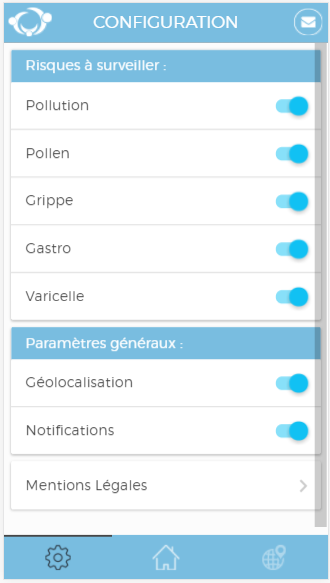
\includegraphics[height=7cm]{figures/subscribe}
	\end{center}
	\caption{Interface Configuration}
	\label{fig4.10}
\end{figure}

Finalement, l'utilisateur peut utiliser les boutons de navigation en bas de l'écran pour consulter les différentes interfaces.Il peut alors solliciter les stations de mesure affichées sur la carte géographique avec le niveau des risques. Il a aussi la possibilité de balayer les risques et les villes. La figure \ref{fig4.11} illustre la rubrique Carte des risques.
\begin{figure}[!h]
	\begin{center}
		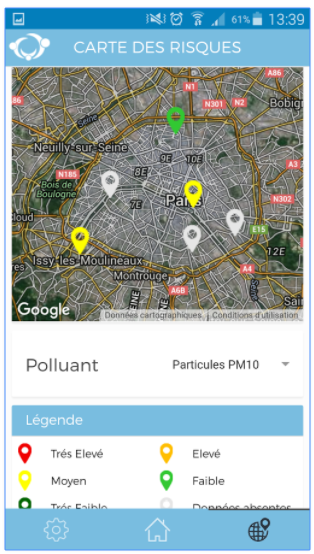
\includegraphics[height=7cm]{figures/station}
	\end{center}
	\caption{Interface Carte des risques}
	\label{fig4.11}
\end{figure}
 
\subsection{Partie: Administrateur}

\qquad L'administrateur a accès à une interface pour visualiser le rapport journalier de l'application. Les informations affichées sont: 
\begin{itemize}
	\item L'historique des notifications
	\item Les villes les plus actives
	\item Les risques les plus consultés
\end{itemize}

L'administrateur peut également télécharger une version xls pour une éventuelle utilisation hors ligne, en cliquant sur le bouton "Export". Le serveur prépare un fichier xls contenant les informations actualisées du rapport, ensuite l'envoie vers la machine de l'administrateur.
La figure \ref{fig4.12} montre l'interface affichée à l'administrateur.

\begin{figure}[!h]
	\begin{center}
		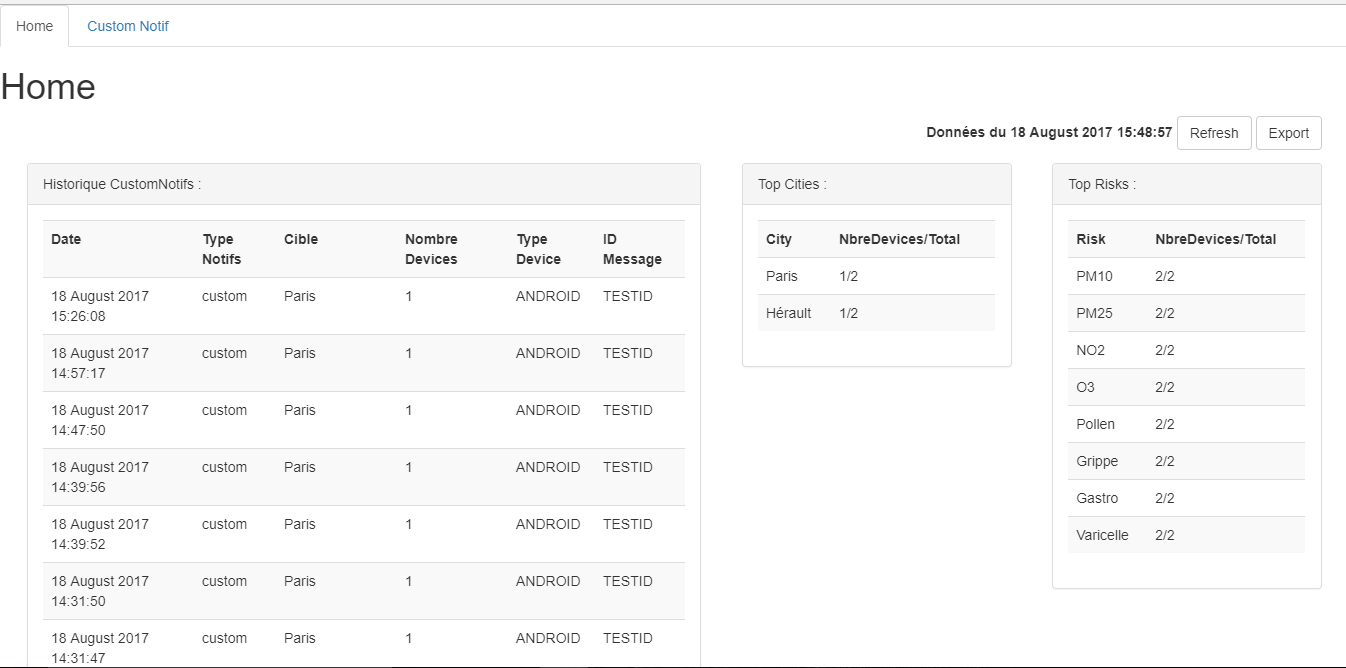
\includegraphics[height=7cm]{figures/admin}
	\end{center}
	\caption{Interface Administration}
	\label{fig4.12}
\end{figure}

L'administrateur peut aussi envoyer des notifications personnaliser aux utilisateurs (voir figure \ref{fig4.13}).

\begin{figure}[!h]
	\begin{center}
		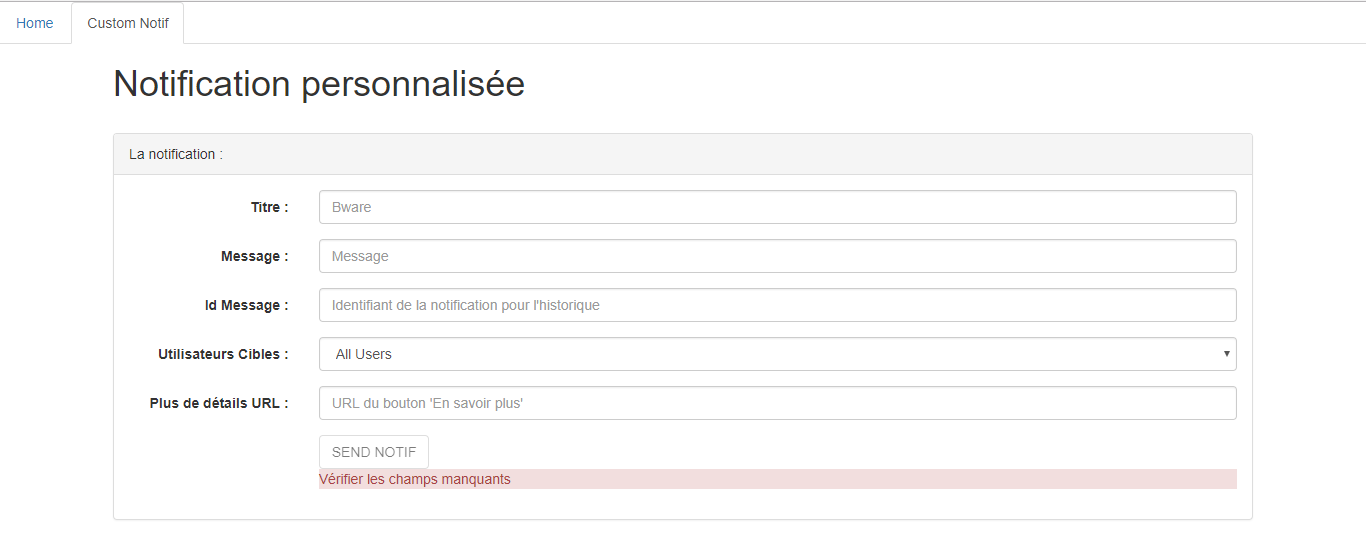
\includegraphics[height=5.5cm]{figures/notif}
	\end{center}
	\caption{Interface Notification personnalisée}
	\label{fig4.13}
\end{figure}

\section{Déploiement et publication de l'application}

\subsection{Déploiement de la partie serveur}
\qquad Les étapes décrites ci-dessous concernent le déploiement en phase de pré-production. Avant de déployer la partie backend dans la machine distante, il faut impérativement préparer le projet à être exécuté dans le nouvel environnement. La différence entre la phase débeugage et la phase production réside majoritairement dans les ressources. Dans la phase débeugage, le serveur Web, le SGBD et l'application cliente existent tous dans la machine du développeur par contre dans la phase pré-production on va séparer chacune de ces parties dans une machine à part comme il est indiqué dans le paragraphe \ref{para}. Cette séparation est effectuée dans le but de tester l'architecture complète avant de la faire passer vers le client final. Pour déployer la partie serveur il faut alors effectuer les étapes suivantes:
\begin{itemize}
	\item Reconfigurer l'application avec les nouvelles adresses et ports utilisés en pré-production (Base de donnée, ports ouverts de l'application...)
	\item Préparer l'application à être exécuté dans le nouvel environnement (Variables d'environnement, variable système...)
	\item Se connecter en Secure Shell (SSH) à la machine distante par la commande
	\begin{itemize}
		\item ssh root@<Adresse IP de la machine>
	\end{itemize}
	\item Éteindre le serveur Web
	\begin{itemize}
		\item /usr/share/tomcat8/bin/shutdown.sh
	\end{itemize}
	\item Supprimer le backup existant et le remplacer par un backup de la version en cours
	\begin{itemize}
		\item rm -rf webapps-smartdata.old
		\item cp -rf webapps-smartdata webapps-smartdata.old
	\end{itemize}
	\item Copier le Web Archive (WAR) vers la machine en utilisant le protocole Secure Copy (SCP) et le placer dans le serveur Tomcat
	\begin{itemize}
		\item scp sd.war root@<Adresse IP de la machine>:/root/documents/2017-07-26
		\item cp /root/document/2017-07-26/sd.war /var/lib/tomcat8/webapps
	\end{itemize}
	\item Redémarrer le serveur Tomcat
	\begin{itemize}
		\item sudo service tomcat8 start; tail -f logs/catalina.out
	\end{itemize}   
\end{itemize} 

\subsection{Publication de l'application dans le play store}

\qquad Pour rendre accessible notre application aux utilisateurs il faut publier celle-ci dans les stores spécifiques à chaque système d'application mobile. Les étapes décrites ci-après concernent la publication dans le play store de Google spécifique à Android. Pour publier l'application mobile dans le store il faut:
\begin{itemize}
	\item Actualiser les informations de configuration de l'application (version, IP du serveur de production...)
	\item Générer une version release de l'application mobile
	\begin{itemize}
		\item ionic cordova build --release android
	\end{itemize}
	\item Générer une clé de signature (il faut l'utiliser pour toute les versions de l'application)
	\begin{itemize}
		\item keytool -genkey -v -keystore release-key.keystore -alias alias\_name -keyalg RSA -keysize 2048 -validity 10000
	\end{itemize}
	\item Signer le binaire avec la clé de signature
	\begin{itemize}
		\item jarsigner -verbose -sigalg SHA1withRSA -digestalg SHA1 -keystore release-key.keystore binary-unsigned.apk alias\_name
	\end{itemize}
	\item Ziper le binaire
	\begin{itemize}
		\item zipalign -v 4 binary-unsigned.apk ready.apk
	\end{itemize}
	\item Télécharger le binaire vers le play store
	\item Publier le binaire dans la forme désirée (Alpha, Beta, Production)
\end{itemize}

\section*{Conclusion}
\qquad Dans ce chapitre, nous avons présenté l’environnement logiciel et matériel dans lequel notre projet a été élaboré. Nous avons ensuite, présenté notre travail à travers un enchaînement de quelques scénarios d’exécution illustrés par des interfaces de l’application. Finalement, nous avons présenté les étapes nécessaires pour déployer notre projet et publier l'application mobile.
